\section{Model Robot}
\label{sec:modelrobot}

\begin{figure} [ht]
  \centering
  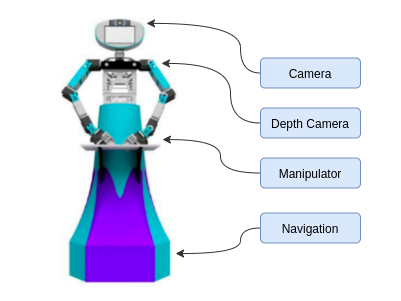
\includegraphics[scale=0.5]{gambar/komponen-robot.png}
  \caption{Diagram komponen pada robot \emph{Dienen}.}
  \label{fig:komponenrobot}
\end{figure}

Robot yang digunakan pada penelitian ini adalah robot \emph{Dienen},
  yang merupakan kelanjutan dari robot \emph{IRIS} \citep{cit:dikairono2020}\citep{cit:zanuar2019} dengan penambahan bagian badan, lengan, dan kepala dari robot \emph{ICHIRO} \citep{cit:muhtadin2019} di bagian atas robot.
Seperti yang terlihat pada Gambar \ref{fig:komponenrobot},
  robot \emph{Dienen} memiliki beberapa komponen yang bisa dikelompokkan menjadi 4 bagian terpisah, yakni sebuah kamera, \emph{depth camera}, \emph{manipulator}, dan \emph{navigation}.

Kamera yang ada pada robot digunakan untuk menangkap citra yang nantinya bisa digunakan untuk melakukan proses visi komputer.
Dengan adanya kamera ini, robot diharapkan mampu memperoleh input untuk melakukan tindakan \emph{assistive} yang bisa berupa deteksi pengguna maupun deteksi objek yang ada di lingkungan.

\emph{Depth camera} yang ada pada robot dapat digunakan untuk menangkap dua macam citra,
  yakni citra berwarna dan citra kedalaman (\emph{depth image}).
Citra gambar yang ditangkap memiliki format RGBA sedangkan citra kedalaman yang ditangkap memiliki format \emph{grayscale} dengan nilai yang semakin gelap menunjukkan jarak yang lebih jauh dari kamera.
\emph{Depth Camera} ini nantinya bisa digunakan untuk melakukan pemetaan ruangan sekaligus meningkatkan keakuratan posisi dan orientasi dari robot menggunakan metode SLAM (\emph{simultaneous localization and mapping}).

\emph{Manipulator} yang ada pada robot terdiri dari dua buah lengan yang memiliki 5 buah \emph{joints} pada masing-masing lengan.
Lengan manipulator ini memiliki sebuah \emph{gripper} di ujung lengan yang dapat digunakan untuk menggenggam sebuah objek.
Dengan adanya lengan manipulator ini,
  robot diharapkan mampu memberikan tindakan \emph{assistive} kepada pengguna seperti membantu untuk membawakan maupun memberikan sebuah objek kepada pengguna.

\emph{Navigation} yang ada pada robot merujuk pada komponen yang memungkinkan pergerakan yang ada pada robot.
Komponen ini terdiri atas tiga buah \emph{omnidirectional wheels} yang terpasang secara \emph{holonomic} sehingga memungkinkan pergerakan ke segala arah,
  dua buah sensor \emph{rotary encoder} yang dapat digunakan untuk memperkirakan posisi dari robot,
  dan sebuah sensor IMU (\emph{inertial measurement unit}) yang dapat digunakan untuk memperkirakan orientasi dari robot.
Dengan adanya komponen Navigasi ini,
  robot diharapkan mampu berpindah tempat secara mudah dari suatu posisi ke posisi yang lain.

\subimport{1-model-robot}{1-model-3d-robot.tex}
\subimport{1-model-robot}{2-struktur-sdf-robot.tex}
